\section{Discussions of theory employed}

\subsection[Exciton complexes]{Exciton complexes and double groups} \label{sec:exciton_theory}
The physical phenomenon which is subject to our study is photoluminiscence. The QDs in a laboratory ensemble are arranged with large spacing and are not expect to interact, hence we can formulate a theoretical model of photoluminiscence on a singular QD. For InGaAs there are two valence bands at the band edge, which are close at $\Gamma$ (see Fig.~\ref{fig:ingaas_band_structure}). These two valence bands have different curvatures at $\Gamma$, and hence correspond to holes of two different effective masses, referred to as heavy holes and light holes.

An external electromagnetic field in the form of a light-beam interacts with the QD in a non-resonant way (as for not to favour a single transition), which promotes electrons into the conduction band and holes into the valence bands. The population of excited electrons and holes of different characteristics is called an exciton complex. Exciton complexes decay into lower-occupancy exciton complexes via electron-hole recombination, which produces bright emission lines in the photoluminiscence spectrum. These lines are sharp and occur at fixed frequencies corresponding to the energy level difference between the initial and final state, and the theoretical description of their spectrum is the ultimate goal of this work.

Exciton complexes are labelled by the number of electron-hole pairs, overall charge, and the occupancy numbers of each hole type. For example, $2X^-_{20}$ has $3$ electrons, $2$ heavy holes, $0$ light holes, and an overall charge of $-1e$.

The excitons with emissions resolvable in the analysed datasets have low occupancy numbers (3 or fewer of any of the three fermions--electrons, light holes, and heavy holes). Because InGaAs has a direct band-gap at $\Gamma$, we approximate the exciton complexes as living on the $\Gamma$ point, i.e. each excited fermion having zero crystal momentum $\vec{k}$ (Fig.~\ref{fig:ingaas_band_structure}). Crystal momentum arises naturally in periodic lattices, since by Bloch's theorem the energy eigenfunctions in a periodic lattice have the form of a function periodic in the lattice modulated by a plane wave of which the associated wavevector $\vec{k}$ is called the crystal momentum vector \cite[Ch.~2.2]{singh}.

\begin{figure}
\begin{center}
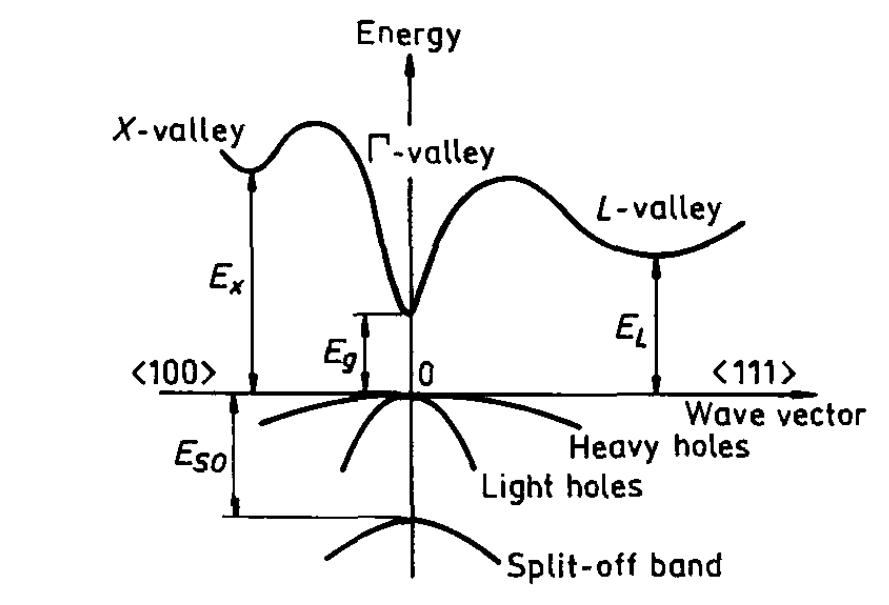
\includegraphics[width=0.7\textwidth]{figures/ingaas_band_structure}
\caption{Band structure of the conduction and valence bands of $\text{In}_{1-x}\text{Ga}_x\text{As}$. In a nanocrystal, the breaking of rotational symmetries may cause the heavy hole and light hole bands to split at $\Gamma$, being no longer degenerate there, as shown in Sec.~\ref{sec:j_coupling}. Figure taken from \cite[Fig.~3.2.1]{semiconductor_handbook} \label{fig:ingaas_band_structure}}
\end{center}
\end{figure}

\subsubsection{Envelope function method} \label{sec:envelopes}
The following approach is informed by that developed by Burt (1999), \cite{envelope_fundamentals}. Let us consider a QD with a single excited electron which is promoted to the conduction band (the following easily generalises to holes promoted to valence bands). Disregarding the spin component of its wavefunction for simplicity, we decompose the electron's spatial wavefunction $\Psi\left(\vec{r}\right)$ into plane-waves:
\begin{equation}
\Psi\left(\vec{r}\right)=\int\dd\vec{k} \tilde{\Psi}\left(\vec{k}\right)\exp{i\vec{k}\vdot\vec{r}}
\end{equation}
where $\tilde{\Psi}\left(\vec{k}\right)$ is the Fourier transform of $\Psi\left(\vec{r}\right)$. From the crystal lattice we construct its reciprocal lattice, the set of vectors $G$ such that a plane wave with a wavevector belonging to $G$ is periodic in the crystal lattice \cite[Ch.~2.6]{singh}. The first Brillouin zone (B.Z.) is then the unit cell of the reciprocal lattice at the origin, and we now decompose the integral domain into the first Brillouin zone summed over the set of reciprocal lattice vectors $G$:
\begin{equation}
\Psi\left(\vec{r}\right)=\sum_{\vec{g}\in G}\int_{\vec{k}\in\text{1st B.Z.}}\dd\vec{k} \tilde{\Psi}\left(\vec{k}+\vec{g}\right)\exp{i\left(\vec{k}+\vec{g}\right)\vdot\vec{r}}
\end{equation}
Note that $G$ is equivalent to the set of wave-vectors of plane waves periodic on the crystal lattice. Therefore, we can choose a set of basis functions $U_n\left(\vec{r}\right)$ periodic on the crystal lattice like so:
\begin{eqnarray}
U_n\left(\vec{r}\right)&=&\sum_{\vec{g}\in G}u_{n}\left(\vec{g}\right)\exp{i\vec{g}\vdot\vec{r}}\\
U_n\left(\vec{r}+\vec{r}_B\right)&=&\sum_{\vec{g}\in G}u_{n}\left(\vec{g}\right)\exp{i\vec{g}\vdot\vec{r}}\exp{i\vec{g}\vdot\vec{r}_B}=U_n\left(\vec{r}\right)
\end{eqnarray}
where $\vec{r}_B\in R$ is a lattice vector and $u_n\left(\vec{g}\right)$ are the coefficients of the decomposition of $U_n$ into reciprocal lattice plane waves, chosen such that $U_n$ are orthonormal. Then, inverting this decomposition, we obtain
\begin{equation}
\exp{i\vec{g}\vdot r} = \sum_n u_n\left(\vec{g}\right)^*U_n\left(\vec{r}\right)
\end{equation}
which allows us to decompose the original wavefunction into a sum of the orthonormal basis vectors $U_n$ and their envelope functions $\Upsilon_n$:
\begin{eqnarray}
\Psi\left(\vec{r}\right)&=&\sum_n \Upsilon_n\left(\vec{r}\right)U_n\left(\vec{r}\right)\\
\Upsilon_n\left(\vec{r}\right)&=&\sum_{\vec{g}\in G}\int_{\vec{k}\in\text{B.Z.}}\dd\vec{k}u_n\left(\vec{g}\right)^*\tilde{\Psi}\left(\vec{k}+\vec{g}\right)\exp{i\vec{k}\vdot\vec{r}}
\end{eqnarray}
Now we choose $U_n\left(\vec{r}\right)$ to represent the band-edge eigenstates in the bulk structure. Using a tight-binding model with spin-orbit coupling, these wavestates can be labelled by three quantum numbers: total angular momentum $j$, its projection onto the $z$-axis $j_z$, and the orbital energy excitation $\varepsilon_n$, which we assume to be in the ground state in our system due to energy occupancy statistics (as we expect the population of states other than in the ground state to be negligible for a low-power light-source). Furthermore, the quantum number $j$ is determined by the orbital angular momentum $l$, which is given by the electron configuration in each specific band, and the spin $s=1/2$ determined for electrons and electron holes by their fundamental properties.

Photonic nanostructures can, on a small scale, cease to posses a standard band-structure, instead featuring e.g. flat bands. Dresselhaus \textit{et al.} (2007) quotes the number of crystal lattice cells below which this occurs to be in the order of $10^2$ \cite[p.~213]{dresselhaus_condensed_matter}. Our QDs have volumes typically higher than $\SI{100}{\nano\metre\cubed}$ \cite[p.~2]{karlsson_2010}, which corresponds to the number of unit cells in the order of $10^3$. Hence we can reasonably expect our system to posses a band structure resembling the standard bulk-lattice band structure in the vicinity of $\Gamma$. This has two consequences to our envelope function model:
\begin{enumerate}
\item The envelope function $\Upsilon\left(\vec{r}\right)$ is varying slowly enough for it to have an approximately defined crystal momentum. As discussed in~\ref{sec:exciton_theory}, we assume $k\approx 0$.
\item The wavefunction $\Psi\left(\vec{r}\right)$ of a single excited fermion approximately corresponds to a single state on the excited band of the band structure of the infinite bulk crystal lattice. In other words, there exists a basis vector $U_n$ such that for all other basis vectors $U_m, m\neq n$, their contribution to the wavefunction is negligible. This postulate is equivalent to disregarding band-mixing effects.
\end{enumerate}
Labelling the single contributing basis vector by the quantum numbers $l, s, j, j_z$, we can express the wavefunction of a single excited fermion as
\begin{equation}
\braket{\vec{r}}{\Psi}=\Upsilon\left(\vec{r}\right)\braket{\vec{r}}{l, s=1/2, j, j_z}
\end{equation}

\subsubsection{Envelope-effective Hamiltonian at $\Gamma$} \label{sec:envelope_effective_hamiltonian}
As discussed by Burt (1992) \cite[p.~6656]{envelope_equation}, we can write down the effective Hamiltonian for the envelope function, which yields the corresponding Schrödinger equation:
\begin{eqnarray}
\hat{H}_\Upsilon &=& -\frac{\hbar^2}{2}\nabla\vdot\frac{1}{m^*\left(\vec{r}\right)}\nabla + E_0\\
\hat{H}_\Upsilon \Upsilon\left(\vec{r}\right)&=& E\Upsilon\left(\vec{r}\right)
\end{eqnarray}
where $E_0$ is the band-edge energy. Now, in a parabolic Taylor expansion of the bands about $\Gamma$, we state that around the $\Gamma$ point the effective mass $m^*$ is constant. We now see that the Schrödinger equation reduces to the following form:
\begin{equation}\label{eq:single_envelope_function}
-\frac{\hbar^2}{2m^*}\nabla^2 \Upsilon = (E-E_0)\Upsilon
\end{equation}
This is the equation of a free particle with energy $E_p=E-E_0$. Hence we can model a single excited fermion as a ``particle in a box'' around the $\Gamma$ point for a large enough structure.

Now we consider the wavefunction of an exciton complex, which is comprised of multiple excited fermions. The interaction between the fermions is purely electromagnetic (disregarding the Pauli exclusion principle, which is treated in Sec. \ref{sec:pauli_exclusion}). Since the envelope functions are slowly-varying and associated to zero crystal momentum, their magnetic interaction is negligible. The magnetic interaction of the periodic basis functions gives rise to spin-orbit and orbit-orbit coupling (ignoring the hyperfine structure of spin-spin coupling), which allows us to label an exciton complex with a total angular momentum $J$ and its projection onto the $z$-axis $J_z$ as two quantum numbers. The Coulomb interaction between fermions $a$ and $b$ gives rise to a term in the Hamiltonian in the form
\begin{equation}
\hat{V}_{ab}^C\left(\vec{r}_a,\vec{r}_b\right)=\frac{q_aq_b}{4\pi\epsilon_0\epsilon_r}\frac{1}{\abs{\vec{r}_a-\vec{r}_b}}
\end{equation}
This operator can be rewritten as a function of a single vector:
\begin{equation}
\hat{V}_{ab}^C\left(\vec{\xi}\right)=\frac{q_aq_b}{4\pi\epsilon_0\epsilon_r}\frac{1}{\xi}, \qq{} \xi = \abs{\vec{\xi}}
\end{equation}
Note that when this operator acts on the full two-particle wavefunction:
\begin{equation} \label{eq:coulomb_interaction_integral}
\hat{V}_{ab}^C\left(\vec{r}_a-\vec{r}_b\right)\Upsilon_a\left(\vec{r}_a\right)U_a\left(\vec{r}_a\right)\Upsilon_b\left(\vec{r}_b\right)U_b\left(\vec{r}_b\right)
\end{equation}
the envelope functions $\Upsilon_a, \Upsilon_b$ are slowly-varying, so we can state that they don't change in the volume of a single crystal lattice cell. Therefore, we can take the envelope functions outside of an integral over a domain where each vector $\vec{r}_a, \vec{r}_b$ is confined to a single cell:
\begin{eqnarray*}
\int_{\vec{r}_a\in \text{cell a}}\dd^3 \vec{r}_a \int_{\vec{r}_b\in \text{cell b}} \dd^3 \vec{r}_b \hat{V}_{ab}^C\left(\vec{r}_a-\vec{r}_b\right)\Upsilon_a\left(\vec{r}_a\right)U_a\left(\vec{r}_a\right)\Upsilon_b\left(\vec{r}_b\right)U_b\left(\vec{r}_b\right) \approx \\
\Upsilon_a\left(\vec{r}_a\right)\Upsilon_b\left(\vec{r}_b\right) \int_{\vec{r}_a\in \text{cell a}}\dd^3 \vec{r}_a \int_{\vec{r}_b\in \text{cell b}} \dd^3 \vec{r}_b \hat{V}_{ab}^C\left(\vec{r}_a-\vec{r}_b\right)U_a\left(\vec{r}_a\right)U_b\left(\vec{r}_b\right)
\end{eqnarray*}
and since $U_a, U_b$ are periodic over the crystal lattice, we can denote $\xi = \vec{R}_{\text{cell b}}-\vec{R}_{\text{cell a}}$ to be the lattice vector equal to the displacement between the two cells, then the integral becomes
\begin{eqnarray*}
\int_{\vec{r}_a\in \text{cell a}}\dd^3 \vec{r}_a \int_{\vec{r}_b\in \text{cell b}} \dd^3 \vec{r}_b \hat{V}_{ab}^C\left(\vec{r}_a-\vec{r}_b\right)\Upsilon_a\left(\vec{r}_a\right)U_a\left(\vec{r}_a\right)\Upsilon_b\left(\vec{r}_b\right)U_b\left(\vec{r}_b\right) \approx \\
\Upsilon_a\left(\vec{r}_a\right)\Upsilon_b\left(\vec{r}_b\right) \int_{\vec{r}_a\in \text{U.C.}}\dd^3 \vec{r}_a \int_{\vec{r}_b\in \text{U.C.}} \dd^3 \vec{r}_b \hat{V}_{ab}^C\left(\vec{r}_a-\vec{r}_b-\vec{\xi}\right)U_a\left(\vec{r}_a\right)U_b\left(\vec{r}_b\right)
\end{eqnarray*}
where U.C. denotes a single unit cell of the crystal lattice centered around the origin (or otherwise fixed in space). Now comes the final approximation. When considering the integral of Eq.~(\ref{eq:coulomb_interaction_integral}) over an arbitrary dual volume, we partition the volumes into unit cells of the crystal lattice and then divide the integral into pairwise U.C.-U.C. integrals over a set of displacement vectors $\vec{\xi}$. For the majority of these vectors in dual volumes comparable in size to the size of the QD, the values of $\xi$ will be larger than the dimensions of the U.C. Hence we can approximate
\begin{equation}
\hat{V}_{ab}^C\left(\vec{r}_a-\vec{r}_b-\vec{\xi}\right)\approx \hat{V}_{ab}^C\left(\vec{\xi}\right)
\end{equation}
By denoting the set of lattice vectors in the volume $V$ as $R_V$, the integral simplifies to
\begin{eqnarray*}
\int_{V}\dd^3 \vec{r}_a\int_{V}\dd^3 \vec{r}_b \hat{V}_{ab}^C\left(\vec{r}_a-\vec{r}_b\right)\Upsilon_a\left(\vec{r}_a\right)U_a\left(\vec{r}_a\right)\Upsilon_b\left(\vec{r}_b\right)U_b\left(\vec{r}_b\right) \approx \\
\Pi_{ab} \sum_{\vec{r}_a\in R_V}\sum_{\vec{r}_b\in R_V} \hat{V}_{ab}^C\left(\vec{r}_a-\vec{r}_b\right)\Upsilon_a\left(\vec{r}_a\right)\Upsilon_b\left(\vec{r}_b\right)\\
\qq{where}\Pi_{ab} = \int_{\vec{r}_a\in \text{U.C.}}\dd^3 \vec{r}_a \int_{\vec{r}_b\in \text{U.C.}} \dd^3 \vec{r}_b U_a\left(\vec{r}_a\right)U_b\left(\vec{r}_b\right) \qq{is a correlation constant.}
\end{eqnarray*}
Now we renormalize the correlation constant $\Pi_{ab}$ using the volume of the unit cell $V_{\text{U.C.}}$, which allows us to rewrite the double sum over $R_V$ as an integral over the dual volume:
\begin{eqnarray*}
\int_{V}\dd^3 \vec{r}_a\int_{V}\dd^3 \vec{r}_b \hat{V}_{ab}^C\left(\vec{r}_a-\vec{r}_b\right)\Upsilon_a\left(\vec{r}_a\right)U_a\left(\vec{r}_a\right)\Upsilon_b\left(\vec{r}_b\right)U_b\left(\vec{r}_b\right) \approx\\
 \Pi'_{ab} \int_{V}\dd^3 \vec{r}_a\int_{V}\dd^3 \vec{r}_b  \hat{V}_{ab}^C\left(\vec{r}_a-\vec{r}_b\right)\Upsilon_a\left(\vec{r}_a\right)\Upsilon_b\left(\vec{r}_b\right),\\
 \qq{where} \Pi'_{ab}=V_{\text{U.C.}}^{-2}\Pi_{ab}=\langle U_a\left(\vec{r}_a\right)U_b\left(\vec{r}_b\right)\rangle_{\text{U.C.}}
 \end{eqnarray*}
 Since this must be true for any (sufficiently large) $V$, we drop the integral altogether, equating the integrands:
 \begin{equation}
 \hat{V}_{ab}^C\left(\vec{r}_a-\vec{r}_b\right) \Psi_a\left(\vec{r}_a\right)\Psi_b\left(\vec{r}_b\right) = \Pi'_{ab}\hat{V}_{ab}^C\left(\vec{r}_a-\vec{r}_b\right)\Upsilon_a\left(\vec{r}_a\right)\Upsilon_b\left(\vec{r}_b\right)\qq{on vol. avg.}
 \end{equation}
 What was done here was essentialy taking a volume average over the product of the basis functions $U_aU_b$, motivated by their periodicity over unit volumes much smaller than that of the quantum dot. This high-frequency periodicity manifests as a simple correlation coefficient when considering matrix elements of $\hat{V}_{ab}^C$.
 
 This allows us to modify Eq.~(\ref{eq:single_envelope_function}) to account for Coulomb interaction purely in the paradigm of envelope functions. The full effective Schrödinger equation for envelope functions (since the fine structure effects do not matter for the slowly-varying envelope functions) is then
 \begin{equation} \label{eq:exciton_envelope_equation}
 \left(-\sum_{i}\frac{\hbar^2}{2m_i^*}\nabla_{\vec{r}_i}^2 +\sum_{i,j; i\neq j} \Pi'_{ij}\hat{V}_{ij}^C\left(\vec{r}_i-\vec{r}_j\right) \right)\Upsilon = E_{\text{exciton}}\Upsilon
 \end{equation}
 where
 \begin{equation*}
 \Upsilon = \prod_{i}\Upsilon_i\left(\vec{r}_i\right)
 \end{equation*}
 Note that the Coulomb interaction on the volumes of the scale of the unit cell of the crystal lattice is fully rotationally symmetric, and therefore will not invalidate $J, J_z$ as good quantum numbers. However, it will affect the value of $\Pi'_{ij}$, which therefore becomes nontrivial to calculate. It will also affect the shape of the periodic functions, which we can for simplicity just denote $F_i\left(\vec{r}_i\right)$, and which have the same periodic properties as $U_i\left(\vec{r}_i\right)$, and form in totality a $J, J_z$ eigenstate. Therefore, we expect the transformation $U_i\to F_i$ to only affect the radial dependence in the close vicinity of an atom, preserving the spherical-harmonics angular dependence in the tight-binding model.
 
 By interpreting Eq.~(\ref{eq:exciton_envelope_equation}), we now see that the envelope functions in an exciton complex behave as free particles in a box with added Coulomb interactions, i.e. a many-body charged particle system. Note that the potential barriers at the edges of the ``box'' are not infinite, and that would indeed not be a good approximation!
 
 \textit{Note.} Even though $\hat{V}_{ab}^C\left(\vec{r}_a-\vec{r}_b\right)$ diverges for $\vec{r}_a=\vec{r}_b$ (which occurs in the small subset of $R_V\otimes R_V$ where both vectors are in the same unit cell), the contribution of the integrals over these coinciding unit cells should not be disproportionally high, since when considering the volume integral in spherical coordinates centered on the asymptote, the integrand goes like $\abs{\vec{r}_a-\vec{r}_b}$, so the integral should be approximately proportional to $V_{\text{U.C.}}^{2/3}$, and the contribution from this subset where our approximations fail to the total integral is negligible.

\subsection{Symmetry in quantum dots} \label{sec:symmetry_arguments}
Now that we have decomposed the single excited fermion wavefunction into a $j$-eigenstate periodic in the atomic lattice and a slowly varying envelope function which corresponds to zero bulk-crystal momentum, we turn to symmetry arguments to make predictions about the spectrum. Indeed, finding either of the two component functions is a task beyond the scope of this work, but we can make quantitative statements about the splitting of the exciton energy levels and selection rules for transitions between these energy levels. To do this, we must consider how the exciton wavefunction transforms under symmetry transformations of the true Hamiltonian.

\subsubsection{Group theory--the formalism of symmetries} \label{sec:group_theory_intro}
A \textit{group} is a set of objects $G$ equipped with a binary operation (here denoted $\cdot$ and referred to as \textit{multiplication}) which satisfies the following requirements \cite[Ch.~1]{dresselhaus}:
\begin{enumerate}
\item \textit{Closure}: If $g_1, g_2$ are elements of $G$, then $g_1\cdot g_2$ is an element of $G$.
\item \textit{Associativity}: The order in which one evaluates multiplication of multiple elements does not matter; $(g_1\cdot g_2) \cdot g_3 = g_1 \cdot (g_2 \cdot g_3)$.
\item \textit{Identity}: There exists a neutral element $e\in G$ such that $e \cdot g = g$ for all $g\in G$.
\item \textit{Inverse}: Each $g\in G$ has its inverse $g^{-1}\in G$ such that $g \cdot g^{-1} = e$.
\end{enumerate}
If a new group can be built on a subset $H$ of the set $G$ under the same operation, it is called a \textit{subgroup} of the group on $G$, denoted $H\subset G$.

A \textit{representation} $\Gamma$ (rep) is a mapping of group elements $g$ onto matrices $D^{(\Gamma)}(g)$ of dimension $\dim\Gamma$ that preserves the group operation as matrix multiplication \cite[Ch.~2]{dresselhaus}:
\begin{equation}
D^{(\Gamma)}(g_1)D^{(\Gamma)}(g_2) = D^{(\Gamma)}(g_1\cdot g_2)
\end{equation}
The \textit{character} of element $g$ in representation $\Gamma$ is the trace of its matrix:
\begin{equation}
\chi^{(\Gamma)}(g)=\Tr D^{(\Gamma)}(g)
\end{equation}
A representation is \textit{reducible} if there exist a similarity transformation which simultaneously brings the matrix of every element into block-diagonal form:
\begin{equation}
D(g)\to P^{-1} D(g) P = \mqty(D_1(g) & 0 \\ 0 & D_2(g))
\end{equation}
When multiplying two block-diagonal matrices of equal structure, the elements from different blocks are decoupled, and hence $D_1(g)$ and $D_2(g)$ form two new, lower-dimensional representations of $G$. A representation which cannot be reduced in this way is called \textit{irreducible} (irrep). There is a finite number of irreps for a finite group, and the tables of their characters for each element for point groups (groups formed on rotations of geometric structures) are included in \cite{altmann}. An example of an irrep is the \textit{identity representation}, for which $D^{\left(\Gamma_I\right)}(g)=1$ for every $g\in G$.

If we restrict a representation of a group to only a subset of elements which forms a subgroup, it is also a representation of the subgroup. In general, irreps may become reducible as representations of the subgroup.

In a vector space where each dimension corresponds to one group element, the characters of an irrep form a vector. These vectors are orthonormal with norm $\sqrt{\abs{G}}$ \cite[Ch.~3]{dresselhaus}. This allows us to uniquely reduce any representation into its constituent irreps, as if decomposing a general vector into a basis.

A set of objects $\ket{\Gamma, i}, i=1,2,\dots \dim \Gamma$ forms a basis to $\Gamma$ if it transforms according to its matrices \cite[Ch.~4]{dresselhaus}:
\begin{equation}
g \mqty(\ket{\Gamma, 1} \\ \ket{\Gamma, 2} \\ \vdots \\ \ket{\Gamma, \dim\Gamma}) = D^{(\Gamma)}(g)\mqty(\ket{\Gamma, 1} \\ \ket{\Gamma, 2} \\ \vdots \\ \ket{\Gamma, \dim\Gamma})
\end{equation}

To review the basic applications of group theory to quantum mechanics \cite[Ch.~5]{dresselhaus}: the set of symmetry transformations $\hat{P}_R$ commuting with a Hamiltonian $\hat{H}$ forms a group under multiplication, denoted $G_{\hat{H}}$, which is referred to as the group of the Hamiltonian. Each energy level $E_n$ of the time-independent Schrödinger eigenvalue problem $\hat{H}\Psi_n=E_n\Psi_n$ corresponds to an irreducible representation of $G_{\hat{H}}$, which we can denote as $\Gamma_{r(n)}$, where $r$ is some mapping. A chosen basis of degenerate eigenstates $\ket{E_n, i}$ is also a basis of $\Gamma_{r(n)}$. The degeneracy of $E_n$ is then equal to the dimension of $\Gamma_{r(n)}$ (assuming no accidental degeneracy). Therefore, knowing the group of the Hamiltonian tells us the possible degeneracies of the energy levels and what they transform as under the symmetry transformations.

Moreover, group theory has an application to selection rules. Consider two energy levels $E_a, E_b$ of a system described by its Hamiltonian $\hat{H}$. If we add a perturbation $\hat{H}'$ which allows transitions between energy levels, and which transforms according to the representation $\Gamma_{\hat{H}'}$, by Fermi's golden rule the rate of transition $E_a\to E_b$ is proportional to the square of the matrix element $\mel{E_a}{\hat{H}'}{E_b}$ \cite[Eq.~(3.2)]{fox}. As per \cite[Ch.~7]{dresselhaus}, this matrix element vanishes if the irrep direct product $\Gamma_{r(a)}\otimes\Gamma_{\hat{H}'}\otimes\Gamma_{r(b)}$ does not contain the identity representation. This allows us to decide which exciton transitions under photoluminiscent electron-hole recombination will be dark in which polarisation.

\subsubsection{Symmetries of quantum dots and double groups}
Consider now the symmetries of the envelope function $\Upsilon=\prod_{i}\Upsilon_i\left(\vec{r}_i\right)$ and the 
periodic function $F=\prod_{i}F_i\left(\vec{r}_i\right)$, respectively.
\begin{enumerate}
\item $\Upsilon$, representing a many-body charged particle-in-a-box system, is governed in its symmetry by the shape of the box, i.e. the shape of the QD. In our system, this shape is assumed to posses $C_{3v}$ (pyramid with equilateral triangle base) symmetry. This symmetry shall be referred to as the \textit{structure symmetry}.
\item $F$, representing a function periodic in the crystal lattice, is governed in its symmetry by the shape of the lattice, i.e. the properties of the bulk of the crystal. In our system, the crystal lattice is a zincblende structure (cubic FCC) \cite[p.~62]{semiconductor_handbook} oriented along the [111] direction. The point group of this lattice is $T_d$ (regular tetrahedron) \cite{zincblende_symmetry}. This symmetry shall be referred to as the \textit{bulk symmetry}.
\item Around the individual atoms in the crystal lattice, in the tight-binding model the exciton forms a total angular momentum eigenstate $\ket{J, J_z}$. This has full roto-inversion symmetry, and since it couples spin-half spinors, which transform according to the fundamental representation of $SU(2)$ under rotations \cite[p.~228]{wigner}, the group describing the full roto-inversion symmetry is $SU(2)\otimes C_i$, where $C_i=\{\hat{E}, \hat{i}\}$ is the inversion group and it is isomorphic to $\mathbb{Z}_2$.
\end{enumerate}
The group of the true Hamiltonian is then constructed from symmetry transformations present in all of these groups. Because the crystal lattice of the QD is oriented along the [111] direction, it contains every structure-symmetry transformation. Therefore the true symmetry is the structure symmetry $C_{3v}$--or rather, since we are considering spin-half spinors, its double group, as will be discussed below. However, as we argue in Sec. \ref{sec:symmetry_suppression}, the bulk symmetry will be important when explaining the origin of symmetry elevation in our perturbative model.

Now, let us consider the character of the full exciton wavefunction under a symmetry transformation $\hat{R}$. Since Coulomb interaction transforms according to the identity rep under roto-inversions (as it depends only on the magnitude of the displacement vector, not its orientation), we can first consider the character of a single fermion wavefunction under the symmetry transformation, and then we construct the full exciton character through $j$-coupling, as discussed in Sec.~\ref{sec:j_coupling}. Since the single excited fermion wavefunction is a product of two functions, its character will be the product of the two constituent characters:
\begin{equation} \label{eq:character_breakdown}
\chi^{\left(\Psi\left(\vec{r}\right)\right)}\left(\hat{R}\right)=\chi^{\left(\Upsilon\left(\vec{r}\right)\right)}\left(\hat{R}\right)\chi^{\left(U\left(\vec{r}\right)\right)}\left(\hat{R}\right)
\end{equation}
The character of the envelope function can be, in principle, any irrep of the structure symmetry group. However, we once again invoke the energy statistics--the population of QDs excited by a low-energy laser for which the envelope functions are out of the ground state should be negligible. Therefore, assuming the envelope function is in its ground state, we know it transforms according to the identity rep. Therefore $\chi^{\left(\Upsilon\left(\vec{r}\right)\right)}\left(\hat{R}\right)=1$.

In the tight-binding model, the band-edge eigenstate $U$ is a convolution of the $j$-eigenstate which exists around each atom with the distribution of the atoms, weighted relatively to their atomic properties. Since the structure symmetry group is a subgroup of the bulk symmetry group, the bulk crystal lattice maps onto itself under every rotation in the structure symmetry. Furthermore, the Ga-As bonds in the conduction band are antisymmetric, and the second-nearest neighbour bonds are symmetric \cite{gaas_bonding}, which leaves the lattice to transform according to the identity rep (Fig.~\ref{fig:zincblende_lattice_structure}).

\begin{figure}
\begin{center}
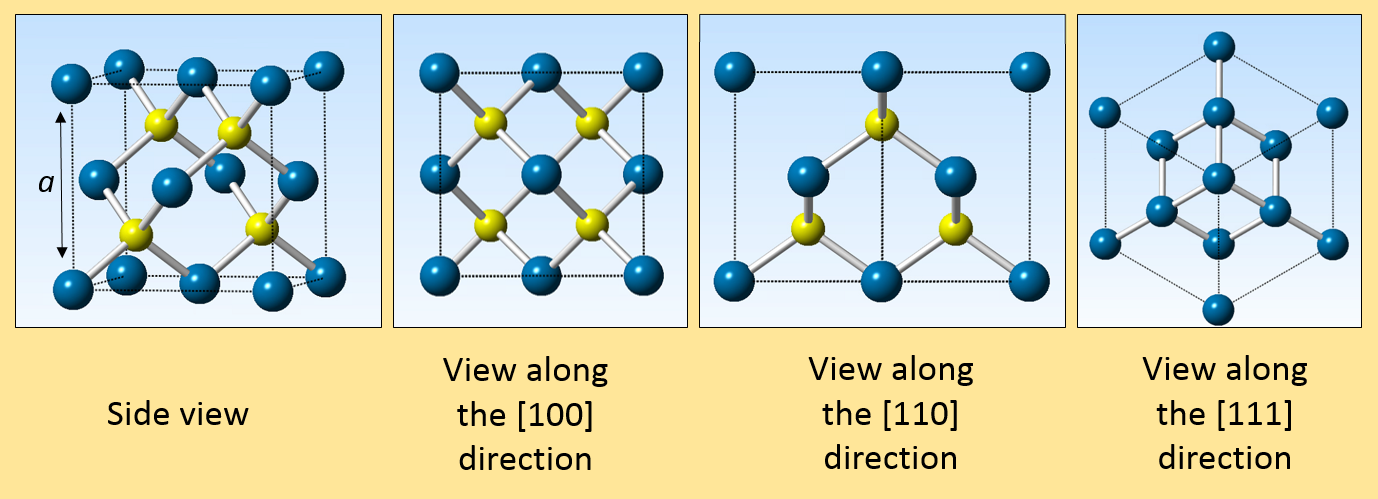
\includegraphics[width=0.9\textwidth]{figures/zincblende_lattice_structure}
\caption{Zincblende lattice structure. Atoms of equal type are second-nearest neighbours, and thus a rotation which maps equal-type atoms onto themselves keeps the lattice-periodic component of the exciton wavefunction constant. Figure taken from \cite[Fig.~2.3]{zincblende_lattice_structure} \label{fig:zincblende_lattice_structure}}
\end{center}
\end{figure}

Therefore the only part of the single excited fermion wavefunction which does not necessarily transform according to the identity rep is the $j$-eigenstate itself. The character of a $j$-eigenstate under any rotation is the trace of the corresponding Wigner $D$-matrix, the general irrep $\Gamma^{(SU(2))}_{j}$ of $SU(2)$ derived by Wigner in \cite[Ch.~15]{wigner} and each set of eigenstates
\begin{equation*}
\mqty(\ket{j,j_z=j}\\\ket{j,j_z=j-1}\\\vdots\\\ket{j, j_z=-j})\mbox{ forms a basis to }\Gamma^{(SU(2))}_{j}
\end{equation*}
To extend this onto roto-inversions, we need to consider the orbital angular momentum $l$, which determines inversion parity. For example, in our system, the conduction band is an $s$-orbital, which has even parity under inversion, but the valence band is a $p$-orbital, which has odd parity under inversion. Determining parity specifies the irrep of the full roto-inversion group $SU(2)\otimes C_i$, which gains an index $g$ (gerade) if even or $u$ (ungerade) if odd under inversion.

Our approach to constructing the transformation laws for the single excited fermions is therefore to consider the irreps of the full roto-inversion spinor group, and then decompose them into the irreps of the true symmetry, i.e. the structure symmetry, which is a process called symmetry breaking \cite[Ch. 6]{dresselhaus}. To do this, we must construct the double group of the structure symmetry point group. Essentially, a double group includes the transformation properties of half-integer $j$ eigenstates, and thus allowing the description of spin-orbit coupling for its original group by adding the time-reversal operator as a generator. Then, rotations by $2\pi$ result in time-reversal, adding a factor of $-1$ to half-integer $j$-eigenstates, and only rotations by $4\pi$ return back to the identity, in agreement with the behaviour of spin-half particles under rotation. The theory of double groups is outlined in \cite[Ch.~19]{dresselhaus}, and the character tables of double groups can be found in standard tables, such as \cite{altmann}.

\subsubsection{Total angular momentum coupling} \label{sec:j_coupling}
To obtain the transformation properties of an exciton complex, we must consider the magnetic orbit-orbit and spin-orbit interaction which couples the total angular momenta $j$ of separate fermions together (Sec.~\ref{sec:envelope_effective_hamiltonian}). The treatment of $j$-coupling in the full roto-inversion symmetry is as follows:

Consider two non-interacting particles governed by Hamiltonians which conserve total angular momentum. Let the two particles exist in $j$-eigenstates $\ket{j^A, j^A_z, p^A}$, $\ket{j^B, j^B_z, p^B}$ respectively (here $p$ specifies the inversion parity), and the group of each of their Hamiltonians is $SU(2)\otimes C_i$. The full Hilbert space they occupy is the direct product of the Hilbert space occupied by each particle, and hence the group of the total Hamiltonian is:
\begin{equation}
G^{\text{non-int.}}_{\hat{H}}=\left(SU(2)\otimes C_i\right)\otimes\left(SU(2)\otimes C_i\right)
\end{equation}
The irreps of this group are the direct products of the respective irreps $\Gamma_{j,p}$, and hence
\begin{equation} \label{eq:noninteracting_j}
\ket{j^A, j^A_z, p^A}\otimes\ket{j^B, j^B_z, p^B}\qq{transforms according to}\Gamma_{j^A, p^A}\otimes\Gamma_{j^B, p^B}
\end{equation}
If we now include an interaction term in the full Hamiltonian which couples the total angular momenta of the particles, $j^A_z, j^B_z$ cease to be good quantum numbers. Instead (in classic electromagnetic coupling), the full total angular momentum $J$ and its projection along the $z$-axis, $J_z$, become good quantum numbers. Preserving $j^A, j^B$ as immutable parameters of the physical system, the new energy eigenstates posses the roto-inversion symmetry $SU(2)\otimes C_i$, and transform according to its irreps. Hence we need to reduce the high-symmetry irrep in Eq.~(\ref{eq:noninteracting_j}) into the lower-symmetry group $SU(2)\otimes C_i$.

We will assume that all constituent irreps in the decomposition have equal parity, which is the product of the two parities $p^A\cdot p^B$. Then, using standard results \cite[Ch.~17]{wigner}, we write down the decomposition:
\begin{equation}
\Gamma_{j^A, p^A}\otimes\Gamma_{j^B, p^B}=\bigoplus_{J=\abs{j^A-j^B}}^{j^A+j^B}\Gamma_{J, p^A\cdot p^B}
\end{equation}
The fact that this equation holds justifies our assumption about coupling inversion parity, since a decomposition is unique.

Using this equation, we see that excited electrons, which couple their intrinsic $s=1/2$ angular momentum to the $l=0$ angular momentum of the conduction band $s$-orbital transform like $\Gamma_{j=1/2, g}$. Similarly, excited holes coupling their $s=1/2$ angular momentum to the $l=1$ angular momentum of the valence band $p$-orbital transform like $\Gamma_{j=1/2, u}\oplus\Gamma_{j=3/2, u}$. The heavy-hole band, the light-hole band, and the split-off band transform as $\ket{3/2, \pm 3/2}$, $\ket{3/2, \pm 1/2}$, $\ket{1/2, \pm 3/2}$, respectively \cite[Eq.~(2.54-56)]{singh}. Identifying $\Gamma_{j=1/2, u}$ as the irrep of the split-off band, which has too small energy to have a hole promote to it instead of to a heavy or light hole band (Fig.~\ref{fig:ingaas_band_structure}), we are left with $\Gamma_{j=3/2, u}$ for the heavy and light holes.

Reducing these representations into the $C_{3v}$ double group, we obtain the irrep $E_{1/2}$ for electrons and the rep $E_{1/2}\oplus E_{3/2}$ for heavy and light holes. Considering how each pair of basis vectors $\ket{3/2, \pm 3/2}$, $\ket{3/2, \pm 1/2}$ transforms under rotations, e.g. by comparing the subtraces of $\Gamma_{j=3/2, u}$ at indices $i=1, 4$ and $i=2,3$, respectively, to the traces of $E_{1/2}$ and $E_{3/2}$, we identify $E_{3/2}$ as the irrep of the heavy-hole band and $E_{1/2}$ as the irrep of the light-hole band. This illustrates that in a nanocrystal with $C_{3v}$ symmetry, the heavy hole and light hole bands undergo splitting, no longer being degenerate at $\Gamma$.

We can now generalise the approach to $j$-coupling to cases where each particle's original Hamiltonian undergoes symmetry breaking to some double group $\tilde{G}_{\hat{H}_0}$, which is a subgroup of $SU(2)\otimes C_i$. In the non-interacting direct product of the two Hilbert spaces, each pair of quantum numbers $j^i, j^i_z$ transforms according to a rep of this subgroup, and so the pair of non-interacting particles transforms according to a rep of $\tilde{G}_{\hat{H}_0}\otimes\tilde{G}_{\hat{H}_0}$. If we include the $j$-coupling interaction term, the full system features only one pair of these quantum numbers, $J, J_z$, which transform according to a rep of the aforementioned subgroup. Hence, the reduction goes like this:
\begin{equation}
\Gamma^{\left(\tilde{G}_{\hat{H}_0}\right)}_A \otimes \Gamma^{\left(\tilde{G}_{\hat{H}_0}\right)}_B \to \bigoplus_i \Gamma^{\left(\tilde{G}_{\hat{H}_0}\right)}_{f(i)}
\end{equation}
where the mapping $f(i)$ specifies the decomposition. Naturally, as the constituent irreps in the direct sum on the right side correspond to different energy levels (disregarding accidental degeneracy), the symmetry breaking associated with coupling of quantum numbers lowers the degeneracy of the system.

\subsubsection{$J$-eigenstate transformations with the Pauli exclusion principle} \label{sec:pauli_exclusion}
The outlined method is sufficient for finding the energy levels of distinguishable particles undergoing coupling; however, in our case, the particles are fermions, and hence, for particles occupying the same $k$-state in the same band, we also have to consider Pauli exclusion principle.

As discussed in Sec.~\ref{sec:j_coupling}, the electrons promoted to the conduction band have $j=1/2$, which renders their $k$-states doubly degenerate, and the holes promoted to the heavy-hole and light-hole valence bands have $j=3/2$ and a $4$-fold degenerate $k$-state at $\Gamma$. However, for certain groups, including $C_{3v}$, the $SU(2)\otimes C_i$ irrep $\Gamma_{j=3/2,u}$ reduces to two $2$-dimensional irreps, which causes light holes and heavy holes to occupy different energy levels at $\Gamma$, each with doubly degenerate $k$-states. We assume that the bands fill up sequentially under excitation in a way that maximises the number of completely filled-up states.
\begin{itemize}
\item For doubly degenerate $k$-states, we only need to find the transformation properties of the full $k$-state, i.e. a pair of fermions. As per Karlsson \textit{et al.} \cite[p.~15]{karlsson}, a full doubly degenerate energy level transforms according to the identity representation.
\item For $4$-fold degenerate $k$-states with $j=3/2$, we can extend Karlsson's argument to claim that the full energy level with $4$ particles transforms according to the identity representation. We can label an energy level with $3$ particles by the $1$ missing particle, and hence it transforms equally to an energy level filled with $1$ particle. Finally, for two particles, we need to construct the $6$ antisymmetric basis vectors, with kets labelled by the $j_z$ values of the first and the second particle respectively:

\begin{center}
\begin{tabular}{ll}
$b_1=\frac{1}{\sqrt{2}}\left(\ket{\frac{3}{2},-\frac{3}{2}}-\ket{-\frac{3}{2},\frac{3}{2}}\right)$ & $b_2=\frac{1}{\sqrt{2}}\left(\ket{\frac{1}{2},-\frac{1}{2}}-\ket{-\frac{1}{2},\frac{1}{2}}\right)$ \vspace{0.2cm}\\
$b_3=\frac{1}{\sqrt{2}}\left(\ket{\frac{3}{2},\frac{1}{2}}-\ket{\frac{1}{2},\frac{3}{2}}\right)$ & $b_4=\frac{1}{\sqrt{2}}\left(\ket{-\frac{3}{2},-\frac{1}{2}}-\ket{-\frac{1}{2},-\frac{3}{2}}\right)$ \vspace{0.2cm}\\
$b_5=\frac{1}{\sqrt{2}}\left(\ket{\frac{3}{2},-\frac{1}{2}}-\ket{-\frac{1}{2},\frac{3}{2}}\right)$ & $b_6=\frac{1}{\sqrt{2}}\left(\ket{-\frac{3}{2},\frac{1}{2}}-\ket{\frac{1}{2},-\frac{3}{2}}\right)$
\end{tabular}
\end{center}

The character of a rotation is given purely by the angle $\theta$, not by the rotation axis, as
\begin{equation} \label{eq:weyl_character}
\chi^{\left(\Gamma_{j}\right)\left(\hat{R}(\theta)\right)}=\frac{\sin{\left(2j+1\right)\theta/2}}{\sin{\theta/2}}
\end{equation}
which is just the trace of the Wigner $d$-matrix, which Wigner defined as
\begin{equation}
d^j_{m',m}=\mel{j,m'}{\hat{R}(\theta)}{j,m}
\end{equation}
where $\theta$ is the second Euler angle in the z-y-z convention \cite[p.~160]{wigner}, and for which Wigner gave an expression \cite[p.~167]{wigner}. The character of a simultaneous rotation of two particles is a product of the two single-particle rotation characters, which allows us to calculate the sum of the simultaneous-rotation characters over all basis vectors:
\begin{equation}
\sum_{i=1}^6 \chi^{b_i}\left(\hat{R}(\theta)\right)=2\cos{\theta}+2\cos{2\theta}+2
\end{equation}
which we can equate to the sum of the characters of $\Gamma_{j=0}\oplus \Gamma_{j=2}$, as per Eq.~(\ref{eq:weyl_character}). Hence an energy level with $j=3/2$ occupied by two particles transforms as $\Gamma_{j=0}\oplus \Gamma_{j=2}$.


\end{itemize}

Hence we can label any exciton complex for groups which have one or two hole characters by labelling each fermion type by the number of free fermions and then multiplying the corresponding representations for each fermion type. Reducing this into the irreps of the structure symmetry group gives the number of energy levels and their degeneracies for each exciton complex (Fig.~\ref{fig:example_labelling}).

\begin{figure}[b]
\begin{eqnarray*}
C_{3v}&&3X_{21}{\xrightarrow{\mbox{  Pauli exc.  }}} \mqty{1\text{ free e.: }E_{1/2}\\0\text{ free hh.: }A_1\\1\text{ free lh.: }E_{1/2}}{\xrightarrow{\qquad}}E_{1/2}\otimes E_{1/2}{\xrightarrow{\mbox{ }j\mbox{-coupling }}}A_1\oplus A_2\oplus E\\
T_d &&2X^-_{11}{\xrightarrow{\mbox{  Pauli exc.  }}} \mqty{1\text{ free e.: }E_{1/2}\\2\text{ free h.: }A_1\oplus E\oplus T_2}{\xrightarrow{\mbox{ }j\mbox{-coupling }}}E_{1/2}\oplus E_{5/2}\oplus F_{3/2}\oplus F_{3/2}
\end{eqnarray*}
\caption{The process of labelling exciton complexes with irreps of the group of the Hamiltonian. $T_d$ has both hole types degenerate at $\Gamma$, and thus they occupy a single quadruply-degenerate energy level (Tab.~\ref{tab:multihole_states}). \label{fig:example_labelling}}
\end{figure}

\subsection[Photoluminiscence spectrum]{Photoluminiscence spectrum and evidence of symmetry elevation}

To predict the rate of photoluminiscent transitions between energy levels, we utilize the dipole approximation, in which the dipole operator (and hence the perturbing Hamiltonian) transforms as a vector \cite[p.~13]{karlsson}. Vectors transform according to the Cartesian representation, which can be easily constructed from rotation matrices \cite[p.~160]{wigner}. If the Cartesian representation is reducible in the structure symmetry group, different vector orientations of the dipole may transform differently, resulting in different lines in polarised spectra. In that case, we must apply the selection rules outlined in Sec.~\ref{sec:group_theory_intro} for each polarisation separately. Then, the number of allowed transitions between different finely-split energy levels of two excitons gives the number of tightly-spaced lines we predict on the spectrum of that exciton transition.

For the assumed symmetry $C_{3v}$, unit vectors $\hat{x},\hat{y}$ transform differently to $\hat{z}$, meaning the spectrum polarised along the $z$-axis will be different than the spectrum polarised in the $x-y$ plane ($\sigma$-polarised). In the experiment, readings for both polarisations are collected utilising a rotatable waveplate \cite[p.~2]{karlsson}.

In \cite{karlsson}, Karlsson \textit{et al.} have applied the selection rules to different exciton transitions and compared the predicted number of lines to their experimental data. The predictions have mostly agreed, but three exciton transitions were identified for which emission lines in the measured spectra were missing (Fig.~\ref{fig:karlsson_elevation_evidence}). These were:
\begin{enumerate}
\item $X_{10}\to $vacuum ($2$ predicted $x-y$-polarised lines, $1$ measured).
\item $2X_{20}\to X_{10}$ ($2$ predicted $x-y$-polarised lines, $1$ measured).
\item $2X_{11}\to X_{01}$ ($6$ predicted $x-y$-polarised lines, $3$ resolved strongly and $2$ more resolved weakly).
\end{enumerate}
Karlsson \textit{et al.} theorise that the missing lines or the relative intensity of lines in these transitions can be explained by a symmetry elevation to a larger group of symmetries of which $C_{3v}$ is a subgroup. In our work, we have attempted to test this claim and identify the mechanism that equips the system with extra symmetries.\\\hfill\\
\makebox[0pt][l]{%
\begin{minipage}{\textwidth}
\centering
    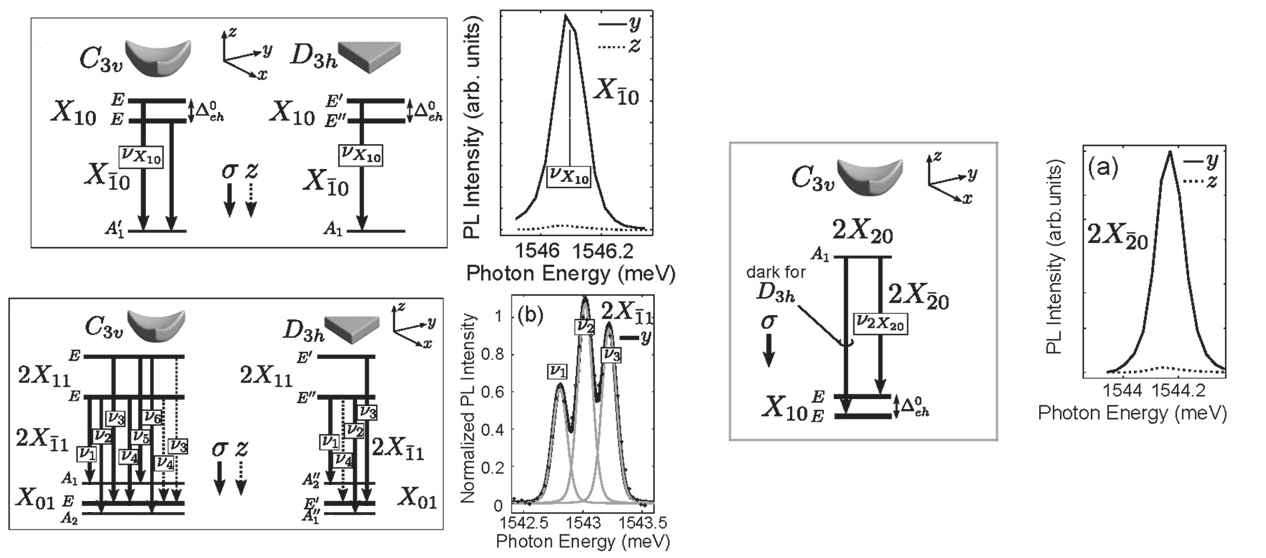
\includegraphics[width=\textwidth]{figures/karlsson_elevation_evidence}
\captionof{figure}{Evidence of symmetry elevation in the research of Karlsson \textit{et al.}, with $D_{3h}$ proposed as the elevated symmetry group. Energy level splitting and allowed transitions for three exciton complexes are plotted for the groups $C_{3v}$ and $D_{3h}$, and identification of emission lines in the spectra is attempted. Figure taken from \cite[Fig.~14, 15, 16]{karlsson} \label{fig:karlsson_elevation_evidence}}
\end{minipage}
}
